\documentclass[uplatex]{jsarticle}
\usepackage[utf8]{inputenc}

\usepackage{amsmath}
\usepackage[dvipdfmx]{graphicx}
\usepackage{resume}  % resume用スタイル
\usepackage{udline}  % 下線用
\usepackage{comment} % 複数行コメント
\pagestyle{plain}
 
\begin{document}
\twocolumn[
    \beginheader{令和5年度 コンピュータサイエンス学部 中中間発表}{2023}{6}{19}{井上 研究室}
    \title{VR環境時の運転シミュレーション酔いの抑制に振動が与える影響}
    \author{C0B20205 武田 夢音 (Yumene Takeda)}
    \endheader
]
\vspace{3mm}

%%ページ番号
\setcounter{page}{9}

\section{はじめに}
近年、VR機器の普及により360度動画の視聴やVRゲームなどのエンターテインメント分野の発展が目覚ましい。これに伴い、子供から高齢者までの幅広い層の使用に耐える品質が求められ、快適性の検討が不可欠となっている。しかし、実際には利用時に違和感を感じたり、眼精疲労、場合によってはめまいや頭痛、吐き気などの「酔い」が起こる問題が生じており、早急な原因究明・対策が望まれている。

酔いの原因については諸説あるが、酔いを良く説明できるものとして感覚不一致説\cite{SensoryConflictTheory}がある。これは、日常の生活で得られる感覚情報パターンは中枢神経内に蓄えられており、船上やVR環境などの普段と異なる感覚情報パターンの環境に置かれた際、中枢神経内で新しい感覚情報パターンへの組み換えが起こると同時に酔いが発生するという説である。

王らは走行中の車体振動を模擬した振動によってドライビング・シミュレータ酔いを抑制する研究を行った\cite{driving_vive}。
この研究は3つのモニタを有するドライビングシミュレータを使用しての実験であり、シートの振動がシミュレータ酔いを抑制することが分かった。
この研究で判明したことは振動がシミュレータ酔いを抑制
するということであり、振動がVR酔いの抑制に影響するかは分かっていない。

\begin{figure}[tb]
  % width や height で絶対的な大きさ指定をすることもできる
  \centering
  \fbox{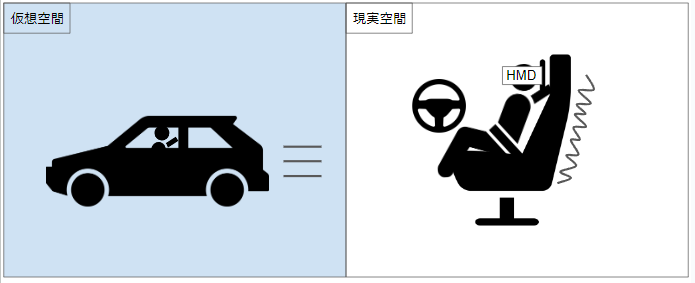
\includegraphics[width=1\linewidth]{fig/about_system.png}}
  \caption{システム概要図}
  \label{fig:about_system}
  \fbox{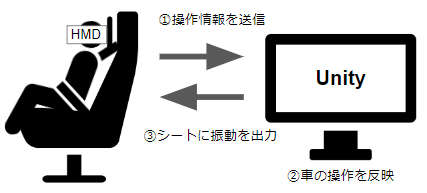
\includegraphics[width=1\linewidth]{fig/system_str.png}}
  \caption{システム構成図}
  \label{fig:system_str}
\end{figure}

\section{関連研究}
王らは走行中の車体振動を模擬した振動によってドライビング・シミュレータ酔いを抑制する研究を行った\cite{driving_vive}。ドライビングシミュレータであるアクセスマスターAM2330には自動車の加減速に応じた座席の振動と、車体振動を模擬した振動を付加する機能があり、これを用いて実験を行った。



\section{VR振動提示システム}
\subsection{システム概要}
システム概要を\figref{fig:about_system}に示す。現実空間にはシートやハンドル、アクセルとブレーキなど実際の車と同じ環境を用意し、VRヘッドセットを装着させる。仮想空間には自動車オブジェクトを用意し、VRヘッドセットの視点はその自動車の運転席に固定する。現実空間での操作に応じて仮想空間内の自動車が動作し、自動車の加減速によってシートに振動が与えられる。

\subsection{システム構成}
システム構成を\figref{fig:system_str}に示す。本システムはHMD、アクセルやブレーキなどの運転機器、振動装置を取り付けたシートから構成される。ユーザはHMDを通して仮想空間を見ており、運転機器の操作状態をUnityに送信する。Unityではそれらの情報を元に仮想空間内の自動車を操作し、操作に応じた振動をシートに与える。





\section{評価方法}
先行研究では評価にSchefféの一対比較法を用いて運転時に感じる「現実感」、「走行感」、「快適さ」を計測していたため、本研究でも同様の評価方法を用いる。

振動を付加した場合としなかった場合の2種類の条件下で1回の運転時間が約3分となるコースを走行させる。

その後、その2条件について実験参加者に評価を求める。

\section{検討事項}
本研究の検討事項は2つある。
1つ目は仮想空間内の自動車の種類である。普通自動車や2輪車、大型トラックなど自動車には種類があるが、現在想定しているのは普通自動車だけであり、他の種類の自動車に対しての実験が必要であるかについて検討が必要である。

2つ目は



\section{まとめ}
本研究ではVR環境での運転シミュレーション酔いに振動が与える影響についての調査を行う。今後はシステム実装と実験を行い、課題を解決できたかを評価する。


 \bibliographystyle{junsrt}
\bibliography{ref.bib}   % 参考文献のデータベースファイルを指定する 
\end{document}
